%11/09 - Patricia Álvarez
\chapter{Modelos de evolución}
Todos los métodos de inferencia y reconstrucción filogenética implican una serie de \textbf{supuestos}, aunque éstos no se hagan explícitos: \begin{itemize}
\item Todos los sitios o posiciones cambian independientemente. 
\item Las tasas de evolución son constantes a lo largo del tiempo y entre linajes.
\item La composición de bases es homogénea.
\item La verosimilitud de los cambios de base es la misma para todos los sitios y no cambia a lo largo del tiempo. 
\end{itemize}

Esto son asunciones, pero en realizar no son ciertos. Las tasas de evolución no son constantes, las posiciones no cambian independientes las unas de las otras, la composición de bases no es homogénea (hay mayor porcentaje de GC que de AT) y se pueden dar múltiples cambios en un único sitio que quedan ocultos (si el nucleótido original es C, puede que en un organismo cambie a A y en otro a G). Estos cambios ocultos hacen que las secuencias estén cada vez más saturadas: la mayoría de los sitios que cambian han cambiado antes. 

En un contexto filogenético, los modelos predicen el proceso de sustitución de las secuencias a través de las ramas. Describen probabilísticamente el proceso por el que los estados de los caracteres homólogos de las secuencias (posiciones alineadas: nucleótidos o aminoácidos) cambian a lo largo del tiempo.

Los modelos implican por lo general los siguientes \textbf{parámetros}: \begin{itemize}
\item \underline{Composición:} frecuencia de las diferentes bases o aminoácidos.
\item \underline{Proceso de sustitución:} tasa de cambio de uno a otro estado de carácter.
\item \underline{Otros parámetros (heterogeneidad de tasas):} proporción de sitios invariables o agregación de los cambios a lo largo de la secuencia.
\end{itemize}

\section{Modelos frecuentes}
El modelo más sencillo es el de Jukes Cantor, el cual asume que todos los cambios son igualmente probables y que la frecuencia de todas las bases es la misma. A partir de este, la complejidad empezó a aumentar, ya que las combinaciones de parámetros son muchas. Algunos de los modelos más frecuentes son: \begin{itemize}
\item \underline{Jukes and Cantor (JC69)}: La frecuencia de todas las bases es la misma (0.25 cada una), y la tasa de cambio de una a otra base es igual.
\item \underline{Kimura 2-parámetros (K2P)}: La frecuencia de todas las bases es la misma (0.25 cada una), pero la tasa de sustitución es diferente para transiciones y transversiones.
\item \underline{Hasegawa-Kishino-Yano (HKY)}: Como K2P, pero la composición de bases varía libremente.
\item \underline{General Time Reversible (GTR)}: La composición de bases varía libremente, y todas las sustituciones posibles pueden tener distintas frecuencias. 
\end{itemize}

Hay programas que ya proponen un modelo a elegir según los datos que se le proporcionen. Cada vez, los modelos son más complejos, y normalmente se utiliza el más complejo. 

%16/09 - Patricia Álvarez
\section{Heterogeneidad de tasas de sustitución}
Los modelos anteriores asumen que el cambio es igualmente probable en todas las posiciones de la secuencia y que la tasa de cambio es constante a lo largo de la filogenia. Pero la intensidad de la selección es rara vez uniforme a lo largo de las posiciones, de modo que lo deseable es \textbf{modelar la variación de las tasas de sustitución sitio por sitio}.

Para una matriz dada, esperamos observar \textbf{posiciones invariables}: \begin{itemize}
\item Porque existen \textbf{restricciones funcionales} (selección purificadora relacionada con la función de los genes).
\item Porque algunas posiciones \textbf{no han tenido ocasión de cambiar}.
\item Debido a \textbf{homoplasias} que hacen que un sitio aparezca como constante.
\end{itemize}

La probabilidad de que un sitio sea invariable puede incluirse en los modelos: la verosimilitud de los datos puede aumentar si consideramos que cierta proporción de los sitios son invariables.

La intensidad de la selección es rara vez uniforme a través de los sitios, de modo que lo deseable es modelar la \textbf{variación de las tasas de sustitución sitio por sitio}. Hay dos posibilidades:
\begin{itemize}
\item Tasa específica de sitio (posición en el codón, alfa-hélices, etc.)
\item Aproximación discreta a una distribución continua (distribución gamma).
\end{itemize}
La \textbf{distribución gamma} se utiliza para modelar la heterogeneidad de las tasas de sustitución entre sitios. La forma de la distribución cambia con diferentes parámetros alfa. Cuanto más bajo es alfa, más concentrados están los cambios en unos pocos sitios. Este parámetro normalmente se calcula por el programa. 

\begin{figure}[htbp]
\centering
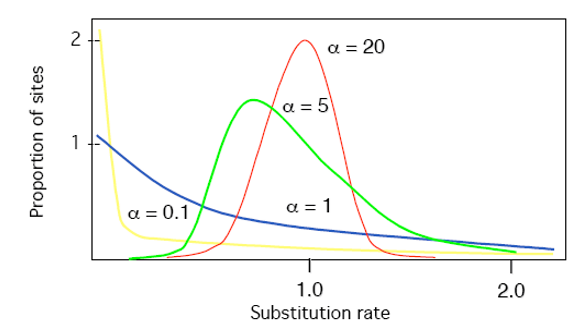
\includegraphics[width=0.5\linewidth]{figs/gamma-distribution.png}
\caption{Formas de distribuciones gamma con diferentes parámetros alfa.}
\end{figure}

\section{Elegir el mejor modelo}
Para obtener el mejor modelo, se suelen utilizar \textbf{métodos probabilísticos}. Los mejores valores para cada parámetro son aquellos que, colectivamente, maximizan la \textbf{verosimilitud de los datos}. La verosimilitud de un modelo es igual a la probabilidad de los datos (como un alineamiento de secuencias) dada una hipótesis de un modelo de evolución molecular.

Para cada modelo, se calcula la verosimilitud de observar los datos si los cambios de secuencia se producen de acuerdo con el modelo. Los modelos serán tanto más complejos cuanto mayor sea el número de parámetros que contemplen. Se comparan unos modelos con otros mediante tests estadísticos (hLRT) o utilizando los criterios de información de Akaike (AIC) o Bayesiano (BIC).

Al añadir parámetros, el modelo se hace más realista. Sin embargo, cada parámetro es estimado a partir de los datos: cuantos más parámetros añadamos, mayor será la varianza de nuestras estimaciones. Por ello, un modelo demasiado “realista” (complejo) puede provocar un excesivo término error, perdiendo potencia estadística. Los criterios de información tienen en cuenta ambas características de los modelos: \begin{itemize}
\item El ajuste del modelo (es mejor el modelo que hace más verosímil observar esos datos).
\item La complejidad del modelo (de dos modelos igualmente verosímiles, el más simple es mejor).
\end{itemize}

\subsection{Selección de esquemas de partición}
Elegir la mejor forma de particionar los datos es casi tan importante como elegir el modelo de sustitución. Distintas partes del alineamiento (posiciones de codón, codificantes frente a no codificantes, etc) pueden ajustarse mejor a diferentes modelos de sustitución o diferentes parámetros de un mismo modelo. Algunas particiones con parámetros de modelos similares pueden combinarse de modo que el número de parámetros final se reduce. La elección del mejor esquema de partición se hace también utilizando criterios de información (AIC y/o BIC). Hay métodos de búsqueda simultánea de los mejores modelos de sustitución y esquemas de partición, como \href{http://www.robertlanfear.com/partitionfinder/}{PartitionFinder}.
